%\renewcommand{\lastmod}{April 29, 2020}

\chapter{Kristallgitter}





\section{Ziele}

\begin{itemize}
\item Sie dewe

\item S.

\end{itemize}


%\begin{figure}
%\inputtikz{\currfiledir fig_bodipy}
%  \caption{Absorptions- und Fluoreszenz-Spektrum des Farbstoffs BODIPY  (\href{https://www.thermofisher.com/de/de/home/life-science/cell-analysis/labeling-chemistry/fluorescence-spectraviewer.html?SID=srch-svtool&UID=10001moh}{thermofischer.com}).}
%\end{figure}



\section{Überblick}

Die Festkörperphysik demonstriert Lösungen für das Problem, ein System aus sehr viele Teilchen einfach zu beschreiben. In der Atomphysik haben wir einen Kern und im Wesentlichen ein Elektron betrachtet. Weitere Elektronen sind hinzu gekommen, deren Wechselwirkung wurde aber quasi vernachlässigt. In der Molekülphysik hatten wir mehrere Atome, oft zwei, manchmal etwa 10. Wieder haben wir das System oft auf die Bewegung einer reduzierten Masse vereinfacht. Im Hückel-verfahren hatten wir eine Methode gesehen, mit der man viele Atome in einem Molekül behandeln kann. In der Festkörperphysik müssen aber nicht ein paar 10 oder 100 Atome, sondern etwa $10^{23}$ Atome behandelt werden. Das Diagonalisieren einer Matrix dieser Kantenlänge ist sicherlich unpraktikabel.

Die Festkörperphysik führt zu diesem Zweck Konzepte zur Behandlung sehr großer Systeme ein. Aus meiner Sicht sind die wesentlichen Konzepte 
\begin{itemize} \setlength{\itemsep}{0pt}
\item das {Kristallgitter}
\item der {reziproke Raum} als Fourier-Transformierte des Kristallgitters
\item das Quasi-Teilchen als Anregung eines Vielteilchen-Systems, die sich wie ein Teilchen benimmt
\item die Dispersionsrelation als Energie-Impuls-Darstellung, die zur Bandstruktur führt
\end{itemize}
In den folgenden vier Kapiteln werden wir diese Konzepte anhand der Kerne in einem Festkörper einführen und deren Effekte diskutieren. Im nächsten Semester in der Festkörperphysik II werden dann Effekte der Elektronen in Festkörpern besprochen werden. Dies ist dann auch das 'modernste' Kapitel der kanonischen Experimentalphysik mit Effekten wie der Supraleitung und dem Quanten-Hall-Effekt.

Wir betrachten hier und im Wesentlichen auch im nächsten Semester nur kristalline, also periodische Festkörper. Man kann die Festkörperphysik als Untermenge der Physik der kondensierten Materie betrachten, in der dann auch amorphe, also nicht-kristalline Festkörper sowie Flüssigkeiten, Gläser und Polymere betrachtet werden. Dies ist dann Thema von Spezialveranstaltungen im Master-Studiengang. 

In diesem Kapitel werden wir die Idee eine Kristallgitters einführen und Methoden zu seiner Beschreibung besprechen. Das sind sozusagen die 'Vokabeln', die wir für die folgenden Kapitel benötigen.


\section{Bravais-Gitter}

Eine Kristallstruktur besteht aus einem mathematischen Punktgitter und einer Basis,  die die Physik in Form von einem oder mehreren Atomen beinhaltet. Man kann sich die Basis als Kachel vorstellen, die entsprechend dem Muster des Punktgitters angeordnet wird. Wie wir sehen werden ist dabei die Wahl der Basis nicht eindeutig. Zunächst betrachten wir nur das mathematische Punktgitter. Dies trägt den Namen von Auguste Bravais.

Ein dreidimensionales (mathematische) Gitter ist eine Anordnung von (mathematischen) Punkten im Raum, die translationsinvariant ist unter jeder Translation $\mathbf{T}$
\begin{equation}
 \mathbf{T} = n_1 \mathbf{a}_1 + n_2 \mathbf{a}_2 + n_3 \mathbf{a}_3  
\end{equation}
wobei die $n_i$ beliebige ganze Zahlen sind und die \emph{Basis-Vektoren} $\mathbf{a}_i$ nicht alle in einer Ebene liegen. Das 'Basis' in diesen Basis-Vektoren hat nichts mit der oben genannten Basis zu tun, die die Physik beinhaltet. Ein beliebiger Vektor aus der Menge der möglichen Translationen $\mathbf{T}$ wird als \emph{Gittervektor} bezeichnet. Die Länge der Basis-Vektoren   $\mathbf{a}_i$, also  $a_i$, wird \emph{Gitterkonstante} genannt.

\begin{marginfigure}
\caption{Primitive und nicht-primitive Basis-Vektoren und Einheitszellen in 2D Gitter}
\end{marginfigure}


Die Wahl der Basis-Vektoren   $\mathbf{a}_i$ ist  bei gegebenem Punktgitter nicht eindeutig. Zum einen sind Linearkombinationen von  Basis-Vektoren ebenfalls möglich, zum anderen verlangt unsere Definition von $\mathbf{T}$ nicht, dass \emph{jeder} Gitterpunkt durch die Translation $\mathbf{T}$  erreicht werden muss.  $\mathbf{a}'_i = 2 \mathbf{a}_i$ ist also ebenfalls möglich. Wir grenzen die Wahl etwas ein, indem wir das durch die Basis-Vektoren   $\mathbf{a}_i$  definierte Volumen betrachten. Dies ist die emph{Elementarzelle} oder \emph{Einheitszelle}. Basis-Vektoren, die das kleinste Volumen aufspannen, nennt man \emph{primitiven Basis-Vektoren} bzw. deren Volumen die \emph{primitive Einheitszelle}. Diese Einheitszelle beinhaltet nur einen Gitterpunkt.\sidenote{Wenn man Punkte an Seiten, Ecken, Kanten der Einheitszelle anteilig rechnet.} Allerdings sind auch die primitiven Basis-Vektoren immer noch nicht eindeutig. Wir werden weiter unten in der Wigner-Seitz-Zelle eine eindeutig definierte primitive Einheitszelle kennenlernen.

\section{Klassifizieren von Bravais-Gittern durch deren Symmetrie}

Wieviel verschiedene Punktgitter kann es im dreidimensionalen Raum geben? Ein Gitter gilt dann als 'verschieden', wenn es eine andere Symmetrie besitzt. Einfach alle Achsen skalieren ändert nichts relevantes. Mögliche Symmetrie-Operationen sind die oben eingeführten Translationen $\mathbf{T}$. Eine andere Art von Symmetrie-Operationen lässt einen einzelnen Gitterpunkt unverändert. Die Menge dieser Operationen nennt man \emph{Punktgruppe} und ist Teil der Gruppentheorie.

\paragraph{Drehung} Was ist der kleinste Winkel $\phi$, um den man ein Gitter drehen kann, so dass es wieder in sich über geht? Dieser Winkel wird in der Form $\phi = 2 \pi / n$ als Zähligkeit $n$ notiert\sidenote{Dies ist die Notation nach Hermann-Mauguin. Alternativ gibt es auch die nach Schoenflies, hier $C_1$, $C_2$ etc.}. Es können nur Werte $n= 1$, 2, 3, 4 und 6 auftreten. Auch im Zweidimensionalen gibt es keine Kacheln mit 5, 7 oder 8 Ecken.

\paragraph{Spiegelung} Bei der Spiegelung an einer Ebene wird nicht nur ein Punkt sonder eine ganze Ebene, in der er liegt, festgehalten. Diese Symmetrie wird durch ein $m$ gekennzeichnet, wenn die Drehachse in dieser Spiegel-Ebene liegt, und durch $/m$, wenn die Drehachse senkrecht auf der Spiegel-Ebene steht.

\paragraph{Inversion} Die Punktspiegelung wird durch $\bar{1}$ gekennzeichnet.

\paragraph{Drehinversion} Dies ist eine hilfreiche zusammengesetzte Symmetrie-Operation aus einer Drehung und anschließender Inversion, die durch die Zähligkeit mit Überstrich, also beispielsweise $\bar{3}$ dargestellt wird. 

Auf Basis der Dreh-Symmetrie können die mathematischen Punkt-Gitter in sieben Klassen unterteilt werden, die sogenannten Kristallsysteme. Im kubischen System gibt es also 4 Rotationsachsen mit jeweils dreizähliger Symmetrie, die vier Raumdiagonalen des Würfels. Die anderen Symmetrie-Operationen werden eine Rolle spielen, wenn wir eine Basis an das mathematische Gitter binden.



\begin{table}
\begin{tabular}{llll}
Kristallsystem 	& 	Symmetrie & Gitterkonstante & Winkel \\
triklin 	&  	$1$						& $a_1 \neq a_2 \neq a_3$ &  $\alpha \neq \beta \neq \gamma$\\
monoklin 	& 	 $2$ 					& $a_1 \neq a_2 \neq a_3$ &  $\alpha = \gamma = 90, \beta \neq 90$\\
orthorhombisch 	& 	  $22$  & $a_1 \neq a_2 \neq a_3$ &  $\alpha= \beta =  \gamma = 90$\\
%
tetragonal 	&  $4$ & $a_1 = a_2 \neq a_3$ &   $\alpha= \beta =  \gamma = 90$\\
trigonal 	& 	 $3$ & $a_1 = a_2 \neq a_3$ &  $\alpha = \beta = 90, \gamma = 120$\\
hexagonal 	& 	  $6$  & $a_1 = a_2 = a_3$ &  $\alpha = \beta = \gamma \neq 90$\\
kubisch 	&  	$3333$  & $a_1= a_2=  a_3$ &  $\alpha= \beta =  \gamma = 90$\\
\end{tabular}
\caption{Die sieben Kristallsysteme. 
 Der Winkel $\alpha$ wird von $\mathbf{a}_2$ und  $\mathbf{a}_3$  eingeschlossen, etc.}
\end{table}


Man kann die sieben Kristallsysteme weiter unterteilen durch Hinzunehmen der Translationssymmetrie $\mathbf{T}$. Effektiv bedeutet dies, dass wo möglich weitere Gitterpunkte hinzugefügt werden, wobei aber die  Rotationssymmtrie der Kristallsysteme erhalten bleibt. 
Dies führt auf die 14 Bravais-Gitter, die in Abbildung \ref{fig:gitter_bravais14} gezeigt sind. Es ist die Leistung von Auguste Bravais zu erkennen, dass es genau diese und keine weiteren mathematisch Punktgitter gibt. Gitter ohne zusätzlioche Punkte werden primitiv genannt, die mit hinzugefügten Oukjten basis-, flächen- oder raum-zentriert. Diese Punkte sind natürlich ebenfalls Gitterpunkte, völlig äquivalent zu den an den Ecken gezeichneten Punkten. Alle Punbkte sind gleich. Man könnte fur die Zeichnung einen anderen Satz Punkte aus der unendlichen Menge der Gitterpunkte herausgreifen, und dann könnten diese Punkte an den Ecken der Darstellung liegen.



\begin{figure}
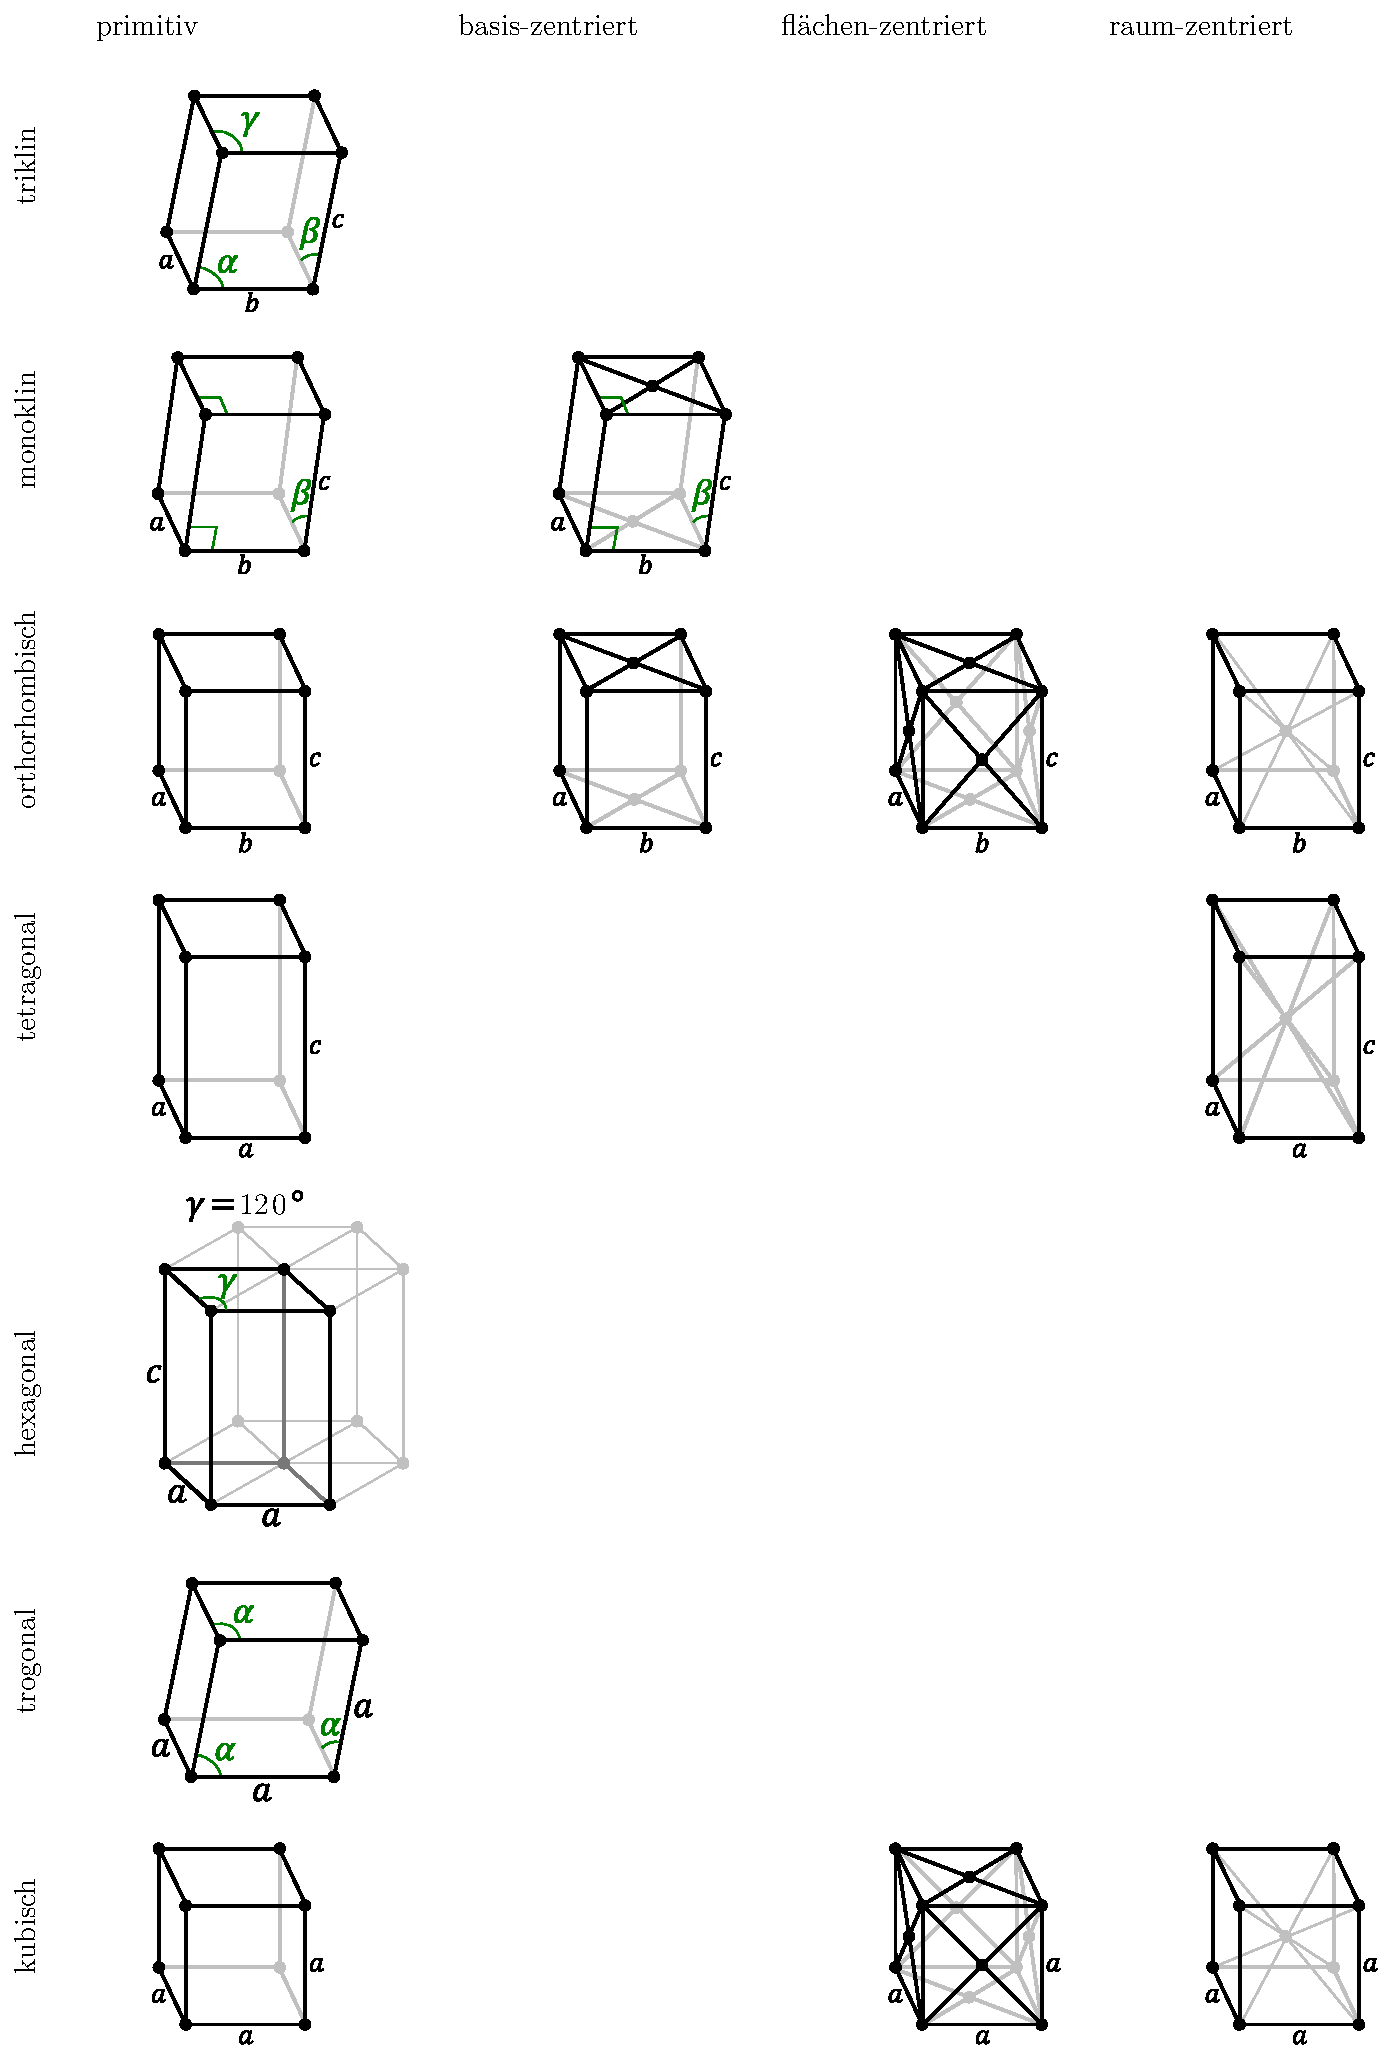
\includegraphics[height=\textheight]{\currfiledir kristall/bravais.pdf}
\caption{Die 14 Bravais-Gitter \label{fig:gitter_bravais14}. Modifiziert nach Wikipedia. Gezeigt ist eine Struktur, die die Symmetrie  des Gitters möglichst gut wiedergibt, nicht die Einheitszelle.
%https://commons.wikimedia.org/wiki/Category:Crystal_system_(image_set) 
}
\end{figure}


\section{Die Basis}


Während das Gitter ein mathematisches Konstrukt ist, eine symmetrische Anordnung von mathematischen Punkten im dreidimensionalen Raum, kommt durch die \emph{Basis} die Natur ins Spiel. Die Basis beschreibt die Position der Atome relativ zum Gitterpunkt. Es kann dabei ein oder mehrere Atome in einer Basis sein. Die Position des Atoms $j$ relativ zum zugehörigen Gitterpunkt ist dann 
\begin{equation}
 \mathbf{r}_j = x_{1,j} \mathbf{a}_1 + x_{2,j} \mathbf{a}_2 + x_{3,j} \mathbf{3}_1  
\end{equation}
mit $0 \le x_{i,j} \le 1$.


Die Symmetrie der Basis hat einen Einfluss auf die Symmetrie des Kristalls. Die sieben Kristallsysteme des mathematischen Gitters werden 32 kristallographische Punktgruppen, wenn also Translationssymmetrie unberücksichtigt bleibt. Diese unterscheiden sich dann in den anderen oben genannten Symmetrie-Operationen.
Wenn wieder die Translationssymmetrie mit berücksichtigen wird ergeben sich 230 kristallographische Raumgruppen.




%-------------------




\printbibliography[segment=\therefsegment,heading=subbibliography]
